\documentclass{article}

\usepackage{arxiv}
\usepackage{amsmath}
\usepackage[utf8]{inputenc} % allow utf-8 input
\usepackage[T1]{fontenc}    % use 8-bit T1 fonts
\usepackage{hyperref}       % hyperlinks
\usepackage{url}            % simple URL typesetting
\usepackage{booktabs}       % professional-quality tables
\usepackage{amsfonts}       % blackboard math symbols
\usepackage{nicefrac}       % compact symbols for 1/2, etc.
\usepackage{microtype}      % microtypography
\usepackage{cleveref}       % smart cross-referencing
\usepackage{lipsum}         % Can be removed after putting your text content
\usepackage{graphicx}
\usepackage{natbib}
\usepackage{doi}
\usepackage{xcolor}
\usepackage{enumerate}% http://ctan.org/pkg/enumerate
\usepackage{booktabs}
% Hyperlinks (load near end to avoid conflicts)
\usepackage{hyperref}                 % Hyperlinks
\hypersetup{
	hidelinks,                        % Hide link boxes
	colorlinks = true,
	citecolor = cyan,
	urlcolor = black,
	linkcolor = magenta
}

\usepackage{subcaption}


\title{Amortized Inference for Spatiotemporal Stochastic Biological Models using Neural Posterior Estimation}

\renewcommand{\shorttitle}{Amortized Inference for Stochastic Models}



% Here you can change the date presented in the paper title
%\date{September 9, 1985}
% Or remove it
%\date{}


% Multiple affiliations variant of author block
\usepackage{authblk}
\renewcommand\Authfont{\bfseries}
\setlength{\affilsep}{0em}
% box is needed for correct spacing with authblk
\newbox{\orcid}\sbox{\orcid}{
\includegraphics[scale=0.06]{orcid.pdf}} 
\author[1]{%
	\href{https://orcid.org/0000-0000-0000-0000}{\usebox{\orcid}\hspace{1mm}Kimpson\thanks{\texttt{kimpson email}}}%
}
\author[1]{%
	\href{https://orcid.org/0000-0000-0000-0000}{\usebox{\orcid}\hspace{1mm}Flegg}}
	
\author[2]{%
	\href{https://orcid.org/0000-0000-0000-0000}{\usebox{\orcid}\hspace{1mm}Simpson}}
	
\author[2]{%
	\href{https://orcid.org/0000-0000-0000-0000}{\usebox{\orcid}\hspace{1mm}Others...}}	

\affil[1]{Unimelb, etc}
\affil[2]{QUT, etc}




% Uncomment to override  the `A preprint' in the header
%\renewcommand{\headeright}{Technical Report}
%\renewcommand{\undertitle}{Technical Report}



\newcommand{\SP}{S\&P2025 }

%%% Add PDF metadata to help others organize their library
%%% Once the PDF is generated, you can check the metadata with
%%% $ pdfinfo template.pdf
%\hypersetup{
%pdftitle={Amortized Inference for Stochastic Biological Models using Neural Posterior Estimation},
%pdfsubject={q-bio.NC, q-bio.QM},
%pdfauthor={David S.~Hippocampus, Elias D.~Striatum},
%pdfkeywords={First keyword, Second keyword, More},
%}

\begin{document}
\maketitle





\begin{abstract}
Parameter inference for stochastic models is essential for quantitative biology, but is hampered by intractable likelihoods. Agent-based random walk models, used widely in ecology and cell biology, exemplify this challenge, often forcing researchers to use likelihood-free methods like Approximate Bayesian Computation (ABC) that introduce biases and tuning difficulties, or else surrogate models which rely on a potentially unfaithful approximation and require an explicit, potentially erroneous, noise model. Here, we overcome these limitations using Neural Posterior Estimation (NPE), a simulation-based, machine learning inference framework that learns the full posterior distribution. Once trained, NPE provides amortized, near-instantaneous posterior estimates. We deploy this framework on a random walk model of a barrier assay experiment. We demonstrate our approach in two settings: first, using one-dimensional summary statistics (column counts), and second, by augmenting NPE with a novel convolutional neural network (CNN) that enables NPE to learn directly from raw two-dimensional spatial data. In both cases, NPE remains the core inference engine, with the CNN serving as a feature extraction component for spatial data. On synthetic data, our NPE pipeline proves highly effective in both settings, delivering posterior estimates at a substantially reduced computational cost per inference. When applied to 1D summary statistics, the pipeline matches or exceeds the precision of classical methods. Similarly, for 2D spatial data, NPE augmented with CNN performs inference directly on raw images with a precision comparable to that from curated summary statistics. This second capability is critical, as it moves beyond the traditional reliance on lower-dimensional data and opens up new avenues for complex models where informative summary statistics are not obvious or available. We provide an open-source implementation of our pipeline to facilitate its adoption and extension to more complex, spatially-structured biological models.
\end{abstract}


% keywords can be removed
\keywords{First keyword \and Second keyword \and More}



\section{Introduction}
Parameter inference is the critical link between mathematical models and biological understanding, enabling quantitative insights from noisy experimental data. Inference methods provide researchers with a powerful toolkit to generate predictions about system behavior, estimate unknown parameters, test competing hypotheses, and rigorously quantify uncertainty. These applications are critical across a wide range of fields, including epidemiology \citep{Dunson2005,Semochkina2025}, ecology \citep{Qian2009,Rosen2001}, cellular biology \citep{Vallejos2015}, gene regulatory networks \citep{Liu2016,Wang2019}, systems biology \citep{Rabinowitz2013} phylogenetics \citep{Nascimento2017}, and neuroscience \citep{Coventry2024}.

For deterministic continuum models described by ordinary and partial differential equations, inference methodologies are mature and well-established. Both Bayesian \citep{Bernardo1994,Gelman1995} and frequentist \citep{Cox1974,Casella1990} approaches provide robust foundations for parameter estimation, model validation, and uncertainty quantification. The sophistication of these inference techniques has enabled reliable parameter estimation and prediction across numerous scientific disciplines including climate science \citep{Vrugt2014}, cosmology \citep{Planck2018Params}, fluid dynamics \citep{Cheung2011} gravitational wave astrophysics \citep{Veitch2015}. 

Stochastic biological models, however, present fundamental inferential challenges that resist these established approaches. Agent-based models and discrete stochastic processes, while capturing essential biological variability and heterogeneity, typically possess intractable likelihoods that preclude standard statistical methods. Experimental protocols exhibit substantial variation, datasets are frequently sparse and noisy, and the stochastic nature of biological processes introduces complex dependencies that deterministic frameworks cannot adequately represent. These characteristics create a disconnect between the sophisticated stochastic models needed to represent biological reality and the inference tools available to calibrate them from data.

Agent-based models of cell migration and proliferation have become a critical testbed for developing new inference techniques that can preserve the biological realism of stochastic models \citep{Carr2021,SIMPSON2022111201,Simpson2025.05.25.656057}. These approaches often use experimental data such as scratch (barrier) assay experiments to calibrate high-fidelity discrete random-walk models, highlighting applications where stochasticity is visible and decision-relevant. At the same time, these successes have clarified several canonical challenges that have historically limited the broader application of stochastic models. While these approaches demonstrate the potential of sophisticated inference frameworks, they also reveal fundamental limitations that must be addressed to fully realize the promise of stochastic biological modeling. These canonical challenges can be summarized as follows. 
\begin{enumerate} 
	\item \textbf{Intractable likelihoods:} The likelihood function for most agent-based models is intractable, precluding the use of standard methods like Maximum Likelihood Estimation or typical Markov chain Monte Carlo (MCMC) algorithms. 
	\item \textbf{Surrogate-model error:} A common strategy to make inference tractable is to replace the computationally expensive stochastic simulator with a cheap surrogate, typically a deterministic Partial Differential Equation (PDE) describing mean-field behavior. While this enables efficient MCMC or MLE techniques, the resulting inference is conditional on the surrogate being a faithful approximation, an assumption that, if violated, can lead to biased parameter estimates and inaccurate predictions. 
	\item \textbf{Noise-model misspecification:} The use of a deterministic surrogate creates the problem of specifying a noise model to connect its clean output to noisy data. A misspecified choice can lead to non-physical predictions and poorly calibrated uncertainties. 
	\item \textbf{Likelihood-free inefficiency:} Classical likelihood-free alternatives like Approximate Bayesian Computation (ABC) are notoriously computationally expensive and sensitive to the choice of summary statistics, distance metrics, and tolerance thresholds.
	\item \textbf{Information loss from summary statistics:} Classical methods often require reducing complex, high-dimensional data (e.g., the full 2D spatial arrangement of cells) to lower-dimensional summary statistics (e.g., a 1D cell density profile). This step risks a significant loss of information, and the choice of statistics can heavily bias the inference. 
	 \end{enumerate}

In this paper, we propose that these fundamental challenges can be addressed in a unified manner using Neural Posterior Estimation (NPE), a modern simulation-based inference (SBI) paradigm. NPE leverages flexible neural density estimators to learn the posterior distribution $p\left(\theta \mid x\right)$ directly from simulator-generated $(\theta,x)$ pairs. This approach offers direct remedies to each of the aforementioned challenges. 
\begin{enumerate} 
	\item It is likelihood-free, circumventing intractability.
	 \item It learns directly from the high-fidelity simulator, eliminating surrogate model bias and removing the PDE as a source of approximation error. 
	 \item It implicitly learns the full, complex, stochastic relationship between parameters and data, obviating the need for an explicit noise model. 
	 \item It can ingest high-dimensional data directly (e.g., raw 2D images), preserving information and avoiding manual selection of summary statistics.
	 \item It provides amortized inference: after an initial, one-time training phase, it can generate posterior estimates for new observations almost instantaneously, overcoming the high per-inference cost of methods like ABC. 
	 \end{enumerate}
The central thesis of this work is that NPE provides a robust, efficient, and direct framework for parameter inference in stochastic biological models. We demonstrate this by applying a state-of-the-art Sequential NPE (SNPE) workflow to a canonical agent-based random walk model of cell migration and proliferation. This type of model is a well-established tool for studying collective cell behaviour \citep[see e.g.][]{Simpson2025.05.25.656057} and serves as an ideal testbed for advanced inference methods. Our main contributions are to: (i) introduce an amortized, simulator-native NPE pipeline for the migration and proliferation random-walk model; (ii) demonstrate that this NPE pipeline circumvents ABC tolerance tuning and surrogate-model bias while improving calibration and coverage; (iii) introduce a novel inference strategy that uses a Convolutional Neural Network (CNN) to learn directly from the raw 2D spatial data generated by the simulator. This approach avoids the information loss inherent in using 1D summary statistics (such as column counts), leading to more precise and reliable posterior estimates; (iv) Release an open, reproducible implementation with configuration files, plots, and posterior-predictive utilities to facilitate adoption and extension. While we use scratch assay experiments as our primary motivating application, the inference framework developed here is applicable to the broader class of spatially-explicit stochastic models commonly used throughout biology and ecology.


The remainder of this paper is structured as follows. Section \ref{sec:classical_inference} reviews the canonical stochastic model and establishes a performance baseline by applying classical inference methods. Section \ref{sec:NPE} details our NPE methodology and demonstrates its performance on one-dimensional summary statistics. Section \ref{sec:results_2d} further enhances this pipeline by embedding a Convolutional Neural Network (CNN) to perform inference directly on raw spatial data. Finally, Section \ref{sec:discussion} discusses the broader implications of our work for the future of simulation-based inference in biology.


\section{Classical Approaches to Inference in Stochastic Biological Models}\label{sec:classical_inference}
Before introducing our NPE framework (Section \ref{sec:NPE}), we briefly review the established approaches to inference for stochastic agent-based models. We draw primarily on the comprehensive treatment in \cite{Simpson2025.05.25.656057} (\SP hereafter), which provides systematic comparisons across multiple inference paradigms for biological random-walk models. These methods have been the workhorses of parameter inference in mathematical biology, each with distinct strengths and limitations that motivate our proposed alternative. Table \ref{tab:method_comparison} provides a comparative overview of these approaches.

\begin{table}[htbp]
	\centering
	\renewcommand{\arraystretch}{1.3} % Increase row spacing
	\begin{tabular}{@{}lcccc@{}}
		\toprule
		\textbf{Method} & \textbf{Cost per Inference} & \textbf{Requires Surrogate?} & \textbf{Requires Summary Stats?} & \textbf{Amortized?} \\
		\midrule
		ABC & Very High & No & Yes & No \\
		Surrogate + MCMC & High & Yes & Yes & No \\
		Surrogate + MLE & Medium & Yes & Yes & No \\
		\textbf{NPE (proposed)} & \textbf{Low\textsuperscript{*}} & \textbf{No} & \textbf{Optional} & \textbf{Yes} \\
		\bottomrule
	\end{tabular}
	\vspace{0.2cm}
	\caption{Comparison of inference approaches for stochastic biological models. \textsuperscript{*}The low cost per inference for NPE is achieved after an initial, computationally intensive training phase.}
	\label{tab:method_comparison}
\end{table}





\subsection{Approximate Bayesian Computation}

Approximate Bayesian Computation (ABC)  represents the most direct approach to likelihood-free inference for stochastic models  \citep{SunnkerABC,Sisson2018}. The foundational ABC rejection sampling algorithm approximates the posterior distribution by undertaking the following steps: (i) a parameter vector $\theta^{(j)}$ is drawn from the prior distribution $p(\theta)$; (ii) a dataset $y^{(j)}$ is simulated from the model using $\theta^{(j)}$; (iii) a discrepancy between the summary statistics of the observed data, $s(y^{\text{obs}})$, and simulated data, $s(y^{(j)})$, is calculated using a distance metric $\rho(\cdot, \cdot)$; and (iv) the parameter $\theta^{(j)}$ is accepted if this discrepancy is less than a tolerance threshold, $\rho(s(y^{\text{obs}}), s(y^{(j)})) \le \epsilon$. The collection of accepted parameters forms a sample from an approximation to the true posterior, $p(\theta \mid y^{\text{obs}})$.


Despite its conceptual simplicity, ABC faces significant methodological and computational challenges. A primary issue is the choice of the tolerance $\epsilon$, which defines a fundamental bias-accuracy trade-off. Only in the idealised limit where $\epsilon \to 0$ and the summary statistics are sufficient does the ABC posterior converge to the true posterior. In practice, a smaller $\epsilon$ reduces bias but dramatically lowers the acceptance rate, increasing computational cost. Conversely, a larger $\epsilon$ increases the acceptance rate at the cost of yielding a more biased and diffuse posterior approximation. 

This trade-off is exacerbated by the "curse of dimensionality". For models with high-dimensional data or parameter spaces, the acceptance rate can be exceptionally low, demanding a vast number of simulations. For instance, S\&P2025 generate $10^5$ simulations from their computationally expensive random walk model to retain just the top 1\%, highlighting this significant computational inefficiency. Furthermore, the method's performance depends critically on the choice of summary statistics. If the statistics are not formally sufficient, crucial information from the data is discarded, which introduces a form of bias that cannot be removed by simply lowering the tolerance $\epsilon$. Selecting informative yet low-dimensional summary statistics in a principled manner remains a difficult and often ad-hoc challenge.



\subsection{Surrogate Model Approaches}
To mitigate the computational burden of methods like ABC, an alternative strategy replaces the stochastic model with a computationally cheaper surrogate model. A common choice is a deterministic partial differential equation (PDE) that captures the system's mean-field behaviour, yielding a tractable likelihood function that enables standard, efficient likelihood-based inference algorithms like Markov Chain Monte Carlo (MCMC). However, this computational gain comes at the cost of introducing potential model misspecification bias, as inference is performed on an approximation of the true stochastic process.

For lattice-based random walk models, the mean behaviour of agents in the continuum limit can be described by a PDE of the form \citep{Codling2008,Simpson2025.05.25.656057,Plank2025}:
\begin{equation}
	\frac{\partial u}{\partial t} = -\frac{\partial J}{\partial x} + S,
\end{equation}
where $u(x,t)$ represents mean agent density, $J$ is the macroscopic flux, and $S$ denotes source terms from proliferation.

The primary limitation of this approach is that the resulting inference is conditional on the fidelity of the surrogate. Any discrepancy between the surrogate and the true stochastic process introduces a systematic bias that cannot be reduced by collecting more data. While the continuum limit accurately describes the mean behaviour of non-interacting random walks, the mean-field PDE neglects crucial stochastic effects in more complex scenarios. For example, in interacting models with crowding effects discussed in S\&P2025 (Section 4), the mean-field approximation captures average behavior but cannot represent the bounded nature of agent occupancy or the discrete stochastic fluctuations around this mean. This limitation becomes particularly important when constructing prediction intervals, where the choice of noise model (e.g. Gaussian vs. binomial, see next Section \ref{sec:noise_model}) significantly affects the physical realism of predictions. These fundamental limitations of surrogate-based approaches motivate the need for inference methods that can work directly with the full stochastic simulator.



\subsubsection{Inference with Surrogate Likelihoods}
A tractable likelihood function from a surrogate model unlocks standard, efficient inference techniques that would be impossible with the original stochastic simulator. These techniques generally fall into two categories: direct optimization or posterior sampling.

The first category, direct optimization, seeks to find the single parameter set that maximizes the likelihood function, yielding the Maximum Likelihood Estimate (MLE). While computationally fast, the MLE provides only a point estimate and does not inherently quantify parameter uncertainty. The second category, posterior sampling, uses methods like Markov Chain Monte Carlo (MCMC) to approximate the full posterior distribution, offering a complete characterisation of uncertainty. However, MCMC typically requires significant computational effort, careful hyperparameter tuning, and rigorous convergence assessment. A third approach, the Laplace approximation, offers a compromise between the speed of optimization and the detailed uncertainty characterization of MCMC. This method approximates the posterior distribution as a multivariate normal distribution centered at the posterior mode (which equals the MLE, $\hat{\theta}$ uner uniform priors). The covariance is given by the inverse of the observed Fisher Information matrix:
\begin{equation}
	p(\theta \mid y^{\text{obs}}) \approx \text{MVN}(\hat{\theta}, \mathcal{I}^{-1}(\hat{\theta})),
\end{equation}
where $\mathcal{I}(\hat{\theta}) = -\nabla\nabla^T \ell(\theta \mid y^{\text{obs}})|_{\theta=\hat{\theta}}$ is the negative Hessian of the log-likelihood evaluated at the mode, often computed using automatic differentiation. While prediction intervals generated via the Laplace approximation can closely match those from more computationally intensive methods (see \SP), the method relies on the assumption that the posterior is locally Gaussian. This assumption may be violated for complex models or with limited data, potentially leading to a poor representation of the true uncertainty. 

However, all these likelihood-based approaches require an explicit specification of how the deterministic surrogate output relates to the noisy observational data—a critical modeling choice we examine next.


\subsection{Noise Model Specification}\label{sec:noise_model}

The use of deterministic surrogates necessitates an explicit choice of how to model the relationship between the clean PDE output and the inherently noisy observations from the stochastic process. This choice profoundly impacts inference results, as the "noise" represents genuine stochastic variability in the agent-based system rather than measurement error. S\&P2025 systematically compares three noise models:

\textbf{Gaussian noise:} The standard assumption that observations are normally distributed around the model prediction with constant variance $\sigma^2$:
\begin{equation}
	N_i | \theta \sim \mathcal{N}(Hu(x_i, t), \sigma^2).
\end{equation}
While mathematically convenient, this leads to unphysical prediction intervals that include negative counts in low-density regions where $u(x,t) \to 0$.

\textbf{Poisson noise:} For count data, a Poisson observation model provides a more natural choice:
\begin{equation}
	N_i | \theta \sim \text{Pois}(Hu(x_i, t)),
\end{equation}
eliminating the additional variance parameter and ensuring non-negative predictions.

\textbf{Binomial noise:} For exclusion processes where occupancy is bounded, the binomial model captures saturation effects:
\begin{equation}
	N_i | \theta \sim \text{Binom}(H, u(x_i, t)).
\end{equation}

S\&P2025's extensive comparisons reveal that noise model misspecification can significantly bias parameter estimates and lead to poorly calibrated prediction intervals. Quantitatively, the Gaussian model consistently produces unphysical negative predictions in low-density regions and encloses only 95\% of data points, while the Poisson and binomial models better respect the discrete, non-negative nature of count data and achieve coverage rates of 99-100\%.




\subsection{Example Results}\label{sec:example_classical_results}
To illustrate these theoretical considerations in practice, we reproduce a representative example from S\&P2025, which focuses on a stochastic agent-based model of a scratch barrier assay. In this model, agents representing biological cells are initially confined to a central region on a two-dimensional lattice and subsequently spread outwards via an unbiased random walk. The resulting spatial distribution is quantified by counting the number of agents in each vertical column, yielding noisy one-dimensional count data. Full details regarding the stochastic model, simulation parameters, and the generation of the synthetic observation can be found in Appendix \ref{sec: synthetic_data_generation}. While S\&P2025 investigates a suite of model variations (e.g., incorporating proliferation and crowding) and alternative PDE approximations, we deliberately focus on this simple case. It provides a clear baseline against which to compare our proposed NPE method, and we refer the reader to the original study for a fuller discussion of these more complex scenarios. We aim to infer two key parameters that govern the model's behaviour: the initial occupation probability, $U$, and an effective diffusion coefficient, $D$. The diffusion coefficient, $D$, is a parameter of the continuum PDE model that can be used as a surrogate. The underlying agent-based model, however, is parameterised by a discrete transition probability, $P$. To facilitate a direct comparison between these different modelling frameworks, we reparameterise the results from the discrete model using the relationship $D=P/4$. We refer the reader to Appendix \ref{sec: synthetic_data_generation} for a full description of the PDE approximation.


Figure \ref{fig:sub1} shows the posterior obtained via ABC. This method operates directly on the stochastic model but relies on one-dimensional summary statistics (column counts), leading to a notably broad posterior. This diffuseness reflects both the inherent stochasticity of the system and the information loss from summarizing the data, showcasing the difficulty in precisely constraining parameters even with a high computational budget. In contrast, Figure \ref{fig:sub2} displays the Gaussian approximation to the posterior (Laplace approximation) derived from maximizing the likelihood of a deterministic surrogate. This approach is computationally efficient and yields a much tighter posterior. However, this apparent precision is entirely conditional on the fidelity of the surrogate; any mismatch between the surrogate and the true stochastic process introduces a systematic bias not reflected in the narrow posterior. Finally, Figure \ref{fig:sub3} shows the posterior sampled using MCMC with the surrogate model and an assumed Gaussian noise model. This provides a more flexible characterization of uncertainty. Crucially, this method requires inferring an additional nuisance parameter, $\sigma$, which quantifies the noise variance. The corner plot shows the joint posterior over the model parameters and this additional noise term. While comprehensive, this result is still fundamentally limited by the choice of surrogate and the specified noise model. 

Collectively, these results highlight the core dilemma: direct methods like ABC are computationally demanding and often imprecise, while surrogate-based methods are faster but introduce hard-to-quantify systematic biases that cannot be reduced by collecting more data.

\begin{figure}[h!]
	\centering
	\begin{subfigure}{0.45\textwidth}
		\centering
		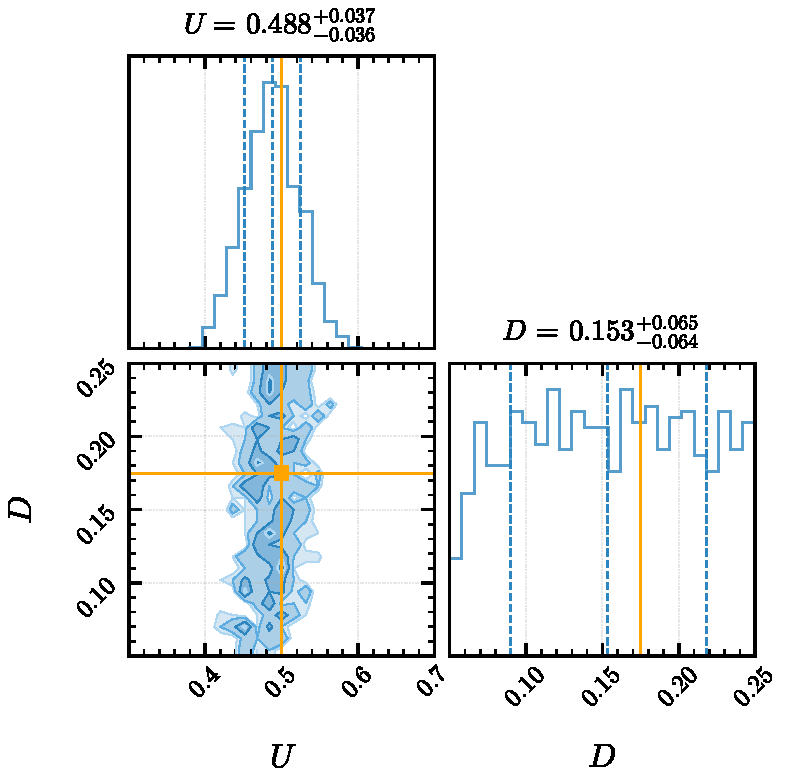
\includegraphics[width=\textwidth]{images/corner_plot_abc_stochastic}
		\caption{Approximate posterior from ABC applied directly to the stochastic model. Computational constraints and information loss lead to a diffuse posterior for $D$}
		\label{fig:sub1}
	\end{subfigure}
	\hfill
	\begin{subfigure}{0.45\textwidth}
		\centering
		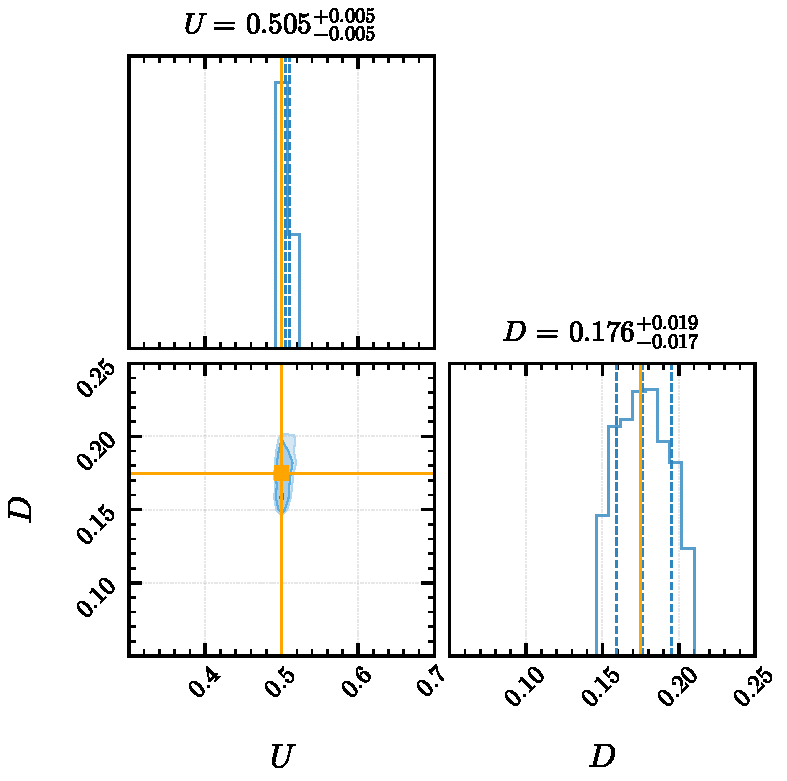
\includegraphics[width=\textwidth]{images/corner_plot_abc_surrogate}
		\caption{Gaussian approximation of the posterior (Laplace approximation) via MLE on a deterministic surrogate model. This approach is computationally efficient but conditional on the surrogate's fidelity.}
		\label{fig:sub2}
	\end{subfigure}
	
	% Add vertical space
	\vspace{1em}
	
	\begin{subfigure}{0.55\textwidth}
		\centering
		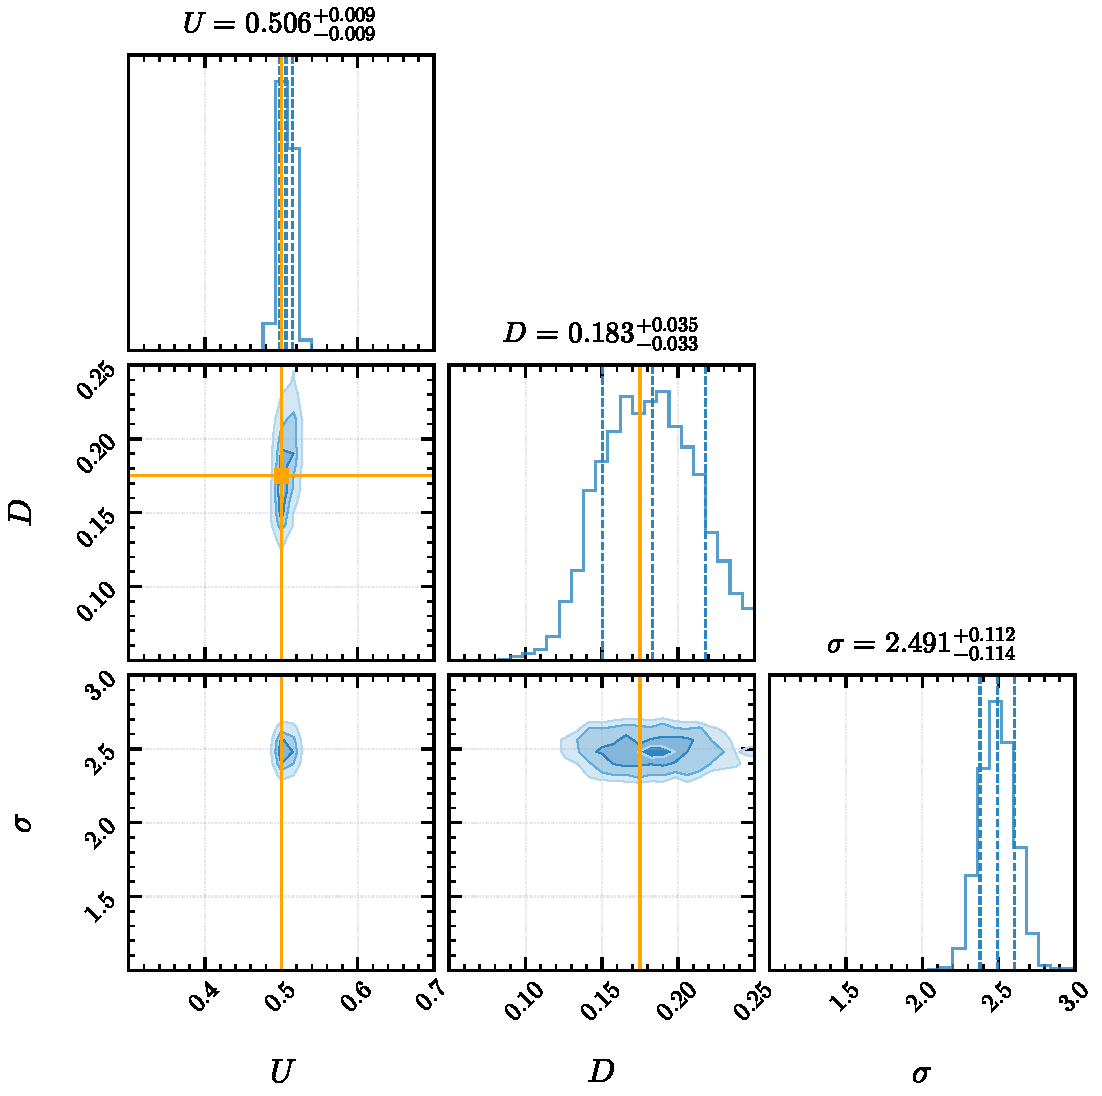
\includegraphics[width=\textwidth]{images/corner_plot_mcmc_surrogate}
		\caption{Posterior distribution from MCMC using the surrogate model with an assumed Gaussian noise model. This method jointly infers the model parameters alongside an additional noise variance parameter, $\sigma$.}
		\label{fig:sub3}
	\end{subfigure}
	\caption{Comparison of posterior distributions obtained using classical inference methods for a scratch assay model. Each approach demonstrates distinct trade-offs between computational efficiency, precision, and model assumptions.}
	\label{fig:three_figures}
\end{figure}

These persistent challenges across classical approaches motivate our exploration of NPE as a unified framework that can address multiple limitations simultaneously through direct learning from simulator output.








\section{Neural Posterior Estimation for Stochastic Biological Models}\label{sec:NPE}

\subsection{Overview and Motivation}
NPE \citep{papamakarios2016fast, greenberg2019automatic,Cranmer2020FrontierSBI} offers a fundamentally different approach to inference for simulator-based models. Rather than relying on surrogate approximations or requiring explicit noise models, NPE learns the posterior distribution $p(\theta | x)$ directly from simulations of the stochastic model. This is achieved through conditional density estimation using neural networks, providing a unified solution to the challenges identified in Section \ref{sec:classical_inference}.

The key insight is that while the likelihood $p(x|\theta)$ may be intractable for complex stochastic simulators, we can still readily generate samples from it by running the simulator. NPE leverages these (parameter, sample) pairs to train a neural network that approximates the inverse mapping — from an observation back to the distribution over parameters that could have produced it. This process is \textit{amortized}; once the network is trained, it can perform posterior inference for any new observation in seconds rather than hours, without requiring additional simulations. For the class of stochastic biological models considered here, this approach directly addresses each limitation of classical methods: it circumvents intractable likelihoods, eliminates surrogate model bias, implicitly captures complex stochastic relationships without explicit noise models, and can process high-dimensional data through automatic feature extraction.

\subsection{Mathematical Foundation}

\subsubsection{Conditional Normalizing Flows}

At the core of NPE are normalizing flows, a class of flexible neural architectures that learn complex probability distributions through invertible transformations. A normalizing flow constructs a target distribution by transforming samples from a simple base distribution (typically a standard Gaussian) through a series of invertible, differentiable mappings.

Formally, let $u \in \mathbb{R}^D$ be a random variable with base density $p_u(u) = \mathcal{N}(0, I)$. The flow defines an invertible transformation $f_\phi: \mathbb{R}^D \rightarrow \mathbb{R}^D$ parameterized by neural network weights $\phi$. For conditional density estimation, this transformation is conditioned on the observation: $\theta = f_\phi(u; x)$. The invertibility requirement ensures that we can both generate samples (forward pass) and evaluate densities (inverse pass). The key insight is that complex distributions can be learned by composing simple transformations, each of which maintains invertibility and efficient Jacobian computation. This allows the network to learn highly flexible posterior shapes while maintaining computational tractability. The resulting approximate posterior density follows from the change of variables formula:
\begin{equation}
	q_\phi(\theta | x) = p_u(f_\phi^{-1}(\theta; x)) \left| \det J_{f_\phi^{-1}}(\theta; x) \right|
\end{equation}
where $J_{f_\phi^{-1}}$ denotes the Jacobian of the inverse transformation. Intuitively, the determinant of the Jacobian corrects for the local change in volume caused by the transformation, ensuring the resulting density is properly normalized. Modern flow architectures (e.g., coupling flows, autoregressive flows) are designed such that this determinant is computationally efficient to calculate.

\subsubsection{Training Procedure}

NPE training requires a dataset of parameter-data pairs generated from the simulator. The training procedure follows three main steps:

\begin{enumerate}
	\item \textbf{Simulation:} Generate $N$ training samples by drawing parameters from the prior $\theta_i \sim p(\theta)$ and simulating corresponding data $x_i \sim p(x|\theta_i)$ using the stochastic model.
	
	\item \textbf{Optimization:} Train the normalizing flow by maximizing the log-likelihood of parameters given their corresponding simulated data:
	\begin{equation}
		\mathcal{L}(\phi) = -\frac{1}{N} \sum_{i=1}^N \log q_\phi(\theta_i | x_i)
	\end{equation}
	
	\item \textbf{Inference:} For observed data $x_o$, obtain the approximate posterior $q_\phi(\theta | x_o)$ by evaluating the trained network. Generate posterior samples by drawing $u \sim p_u(u)$ and applying the learned transformation $\theta = f_\phi(u; x_o)$.
\end{enumerate}
The training data requirements scale with problem complexity, but it is difficult in general to provide quantitative reccomendation on the number of required simulations to train the model. Typically at least $N = 10^4 - 10^6$ simulations suffice for moderate-dimensional parameter spaces ($d \leq 10$), though higher-dimensional problems may require larger datasets \citep{2025arXiv250812939D}. Crucially, this procedure is \textit{amortized}; the computationally expensive training phase is performed only once, after which posterior inference for any new observation is nearly instantaneous. This represents a significant advantage over methods like ABC, which require fresh simulations for each new dataset.

\subsection{Sequential Neural Posterior Estimation}

While the basic NPE algorithm is powerful, it can be inefficient when the prior is much broader than the posterior. Sequential Neural Posterior Estimation (SNPE) \citep{papamakarios2016fast, greenberg2019automatic} addresses this through an iterative refinement process that concentrates computational effort on parameter regions consistent with the observed data.

The sequential algorithm proceeds as follows:

\begin{enumerate}
	\item \textbf{Round 1:} Train an initial density estimator using simulations from the prior, obtaining $q_{\phi_1}(\theta | x)$.
	
	\item \textbf{Subsequent rounds $(r > 1)$:} Use the posterior approximation from round $r-1$ evaluated at the observed data, $q_{\phi_{r-1}}(\theta | x_o)$, as a proposal distribution. Generate new simulations $\theta \sim q_{\phi_{r-1}}(\theta | x_o)$, $x \sim p(x|\theta)$.
	
	\item \textbf{Importance weighting correction:} Train a new density estimator $q_{\phi_r}(\theta | x)$ on the focused simulations, with importance weighting to correct for the proposal distribution bias:
	\begin{equation}
		\mathcal{L}_r(\phi) = -\frac{1}{N_r} \sum_{i=1}^{N_r} w_i \log q_\phi(\theta_i | x_i)
	\end{equation}
	where $w_i = p(\theta_i) / q_{\phi_{r-1}}(\theta_i | x_o)$ corrects for sampling from the proposal rather than the prior.
\end{enumerate}

SNPE is most beneficial when the prior is substantially broader than the posterior, which is common in biological applications where parameter ranges are often set conservatively. The method typically converges within 2-4 rounds, providing substantial efficiency gains over standard NPE while maintaining accuracy. In this work we will exclusively use the sequential version of NPE.

\subsection{Implementation Details}

All NPE analyses in this work use the \texttt{sbi} Python package \cite{2020JOSS....5.2505T}, which provides a well-documented implementation of state-of-the-art simulation-based inference algorithms. We employ neural spline flows \cite{durkan2019neural} as our density estimator architecture, which offer excellent expressivity while maintaining computational efficiency. Additional implementation details are presented in Appendix \ref{ap:npe_implementaion}



\subsection{Application to Barrier Assay Data: 1D Column Count Analysis} \label{sec:1d_results}

We demonstrate NPE's effectiveness by applying it to the same synthetic barrier assay data used in Section \ref{sec:example_classical_results}. To ensure direct comparison with the classical methods, we first implement NPE using identical 1D column count summary statistics $N_i$, representing the number of agents in each vertical column of the lattice. In Section \ref{sec:results_2d} we will extend this to operate directly on the 2D spatial data.

\subsubsection{Experimental Setup}
Following the protocol of \SP, we generate synthetic observations from a stochastic random walk model with true parameters $P = 0.7$ and $U = 0.3$, corresponding to diffusivity $D = P/4 = 0.175$ in the continuum limit. The resulting data consists of a 201-dimensional vector of column counts. We perform inference directly on the stochastic model parameters $P$ and $U$, then transform to $D$ via the relationship $D = P/4$ for comparison with PDE-based approaches. We use  broad uniform priors covering the full parameter space: $P \sim \mathcal{U}(0.0, 1.0)$ and $U \sim \mathcal{U}(0.01, 1.0)$.


\subsubsection{Parameter Inference Results}
Figure \ref{fig:npe_1d_posterior} presents the posterior distribution obtained via NPE. NPE recovers a posterior distribution with means $P = 0.698 \pm 0.037$ and $U = 0.301 \pm 0.022$ (mean $\pm$ standard deviation), corresponding to $D = 0.175 \pm 0.009$ after transformation. The results demonstrate excellent agreement with the true parameter values ($P = 0.7$, $U = 0.3$) 

This approach yields several key advantages over classical methods. The NPE posterior shows substantially improved precision, than a posterior obtained from a comparable ABC analysis, especially for the diffusion paramter $D$, all without the need for manual tolerance tuning. Furthermore, because NPE learns directly from the stochastic simulator, it avoids the systematic bias of mean-field approximations and produces a posterior that is not artificially narrow. The resulting credible intervals accurately reflect the natural stochastic variance of the data, a feature often lost when using deterministic surrogate models. Once the initial network training is complete, posterior samples for any new observation can be obtained almost instantly.
\begin{figure}[h]
	\centering
	\includegraphics[width=0.8\textwidth]{images/NPE_corner_plot_1d_D}
	\caption{Posterior distribution from NPE using 1D column count data. The contours show 68\% and 95\% credible regions, with the true parameter values (organge cross) falling well within the high-probability region.}
	\label{fig:npe_1d_posterior}
\end{figure}


\subsubsection{Predictive Performance}\label{sec:posterior_checks}

Beyond parameter estimation, we evaluate NPE's predictive capabilities through posterior predictive sampling. For each posterior sample $\theta^{(j)}$, we generate predicted data $\tilde{x}^{(j)} \sim p(x|\theta^{(j)})$ using the stochastic simulator. The collection of predictions forms empirical prediction intervals that naturally account for both parameter uncertainty and model stochasticity.

The resulting NPE-based predictions are well-calibrated, with 94.8\% of true observations falling within the 95\% prediction intervals. A key advantage of this simulator-native approach is its physical consistency; the prediction intervals respect the non-negative, discrete nature of the count data without requiring an explicit, and potentially erroneous, noise model. Furthermore, the framework naturally captures heteroscedastic uncertainty, with the prediction intervals appropriately widening in regions of high agent density where stochastic variability is greatest.

\begin{figure}[h]
	\centering
	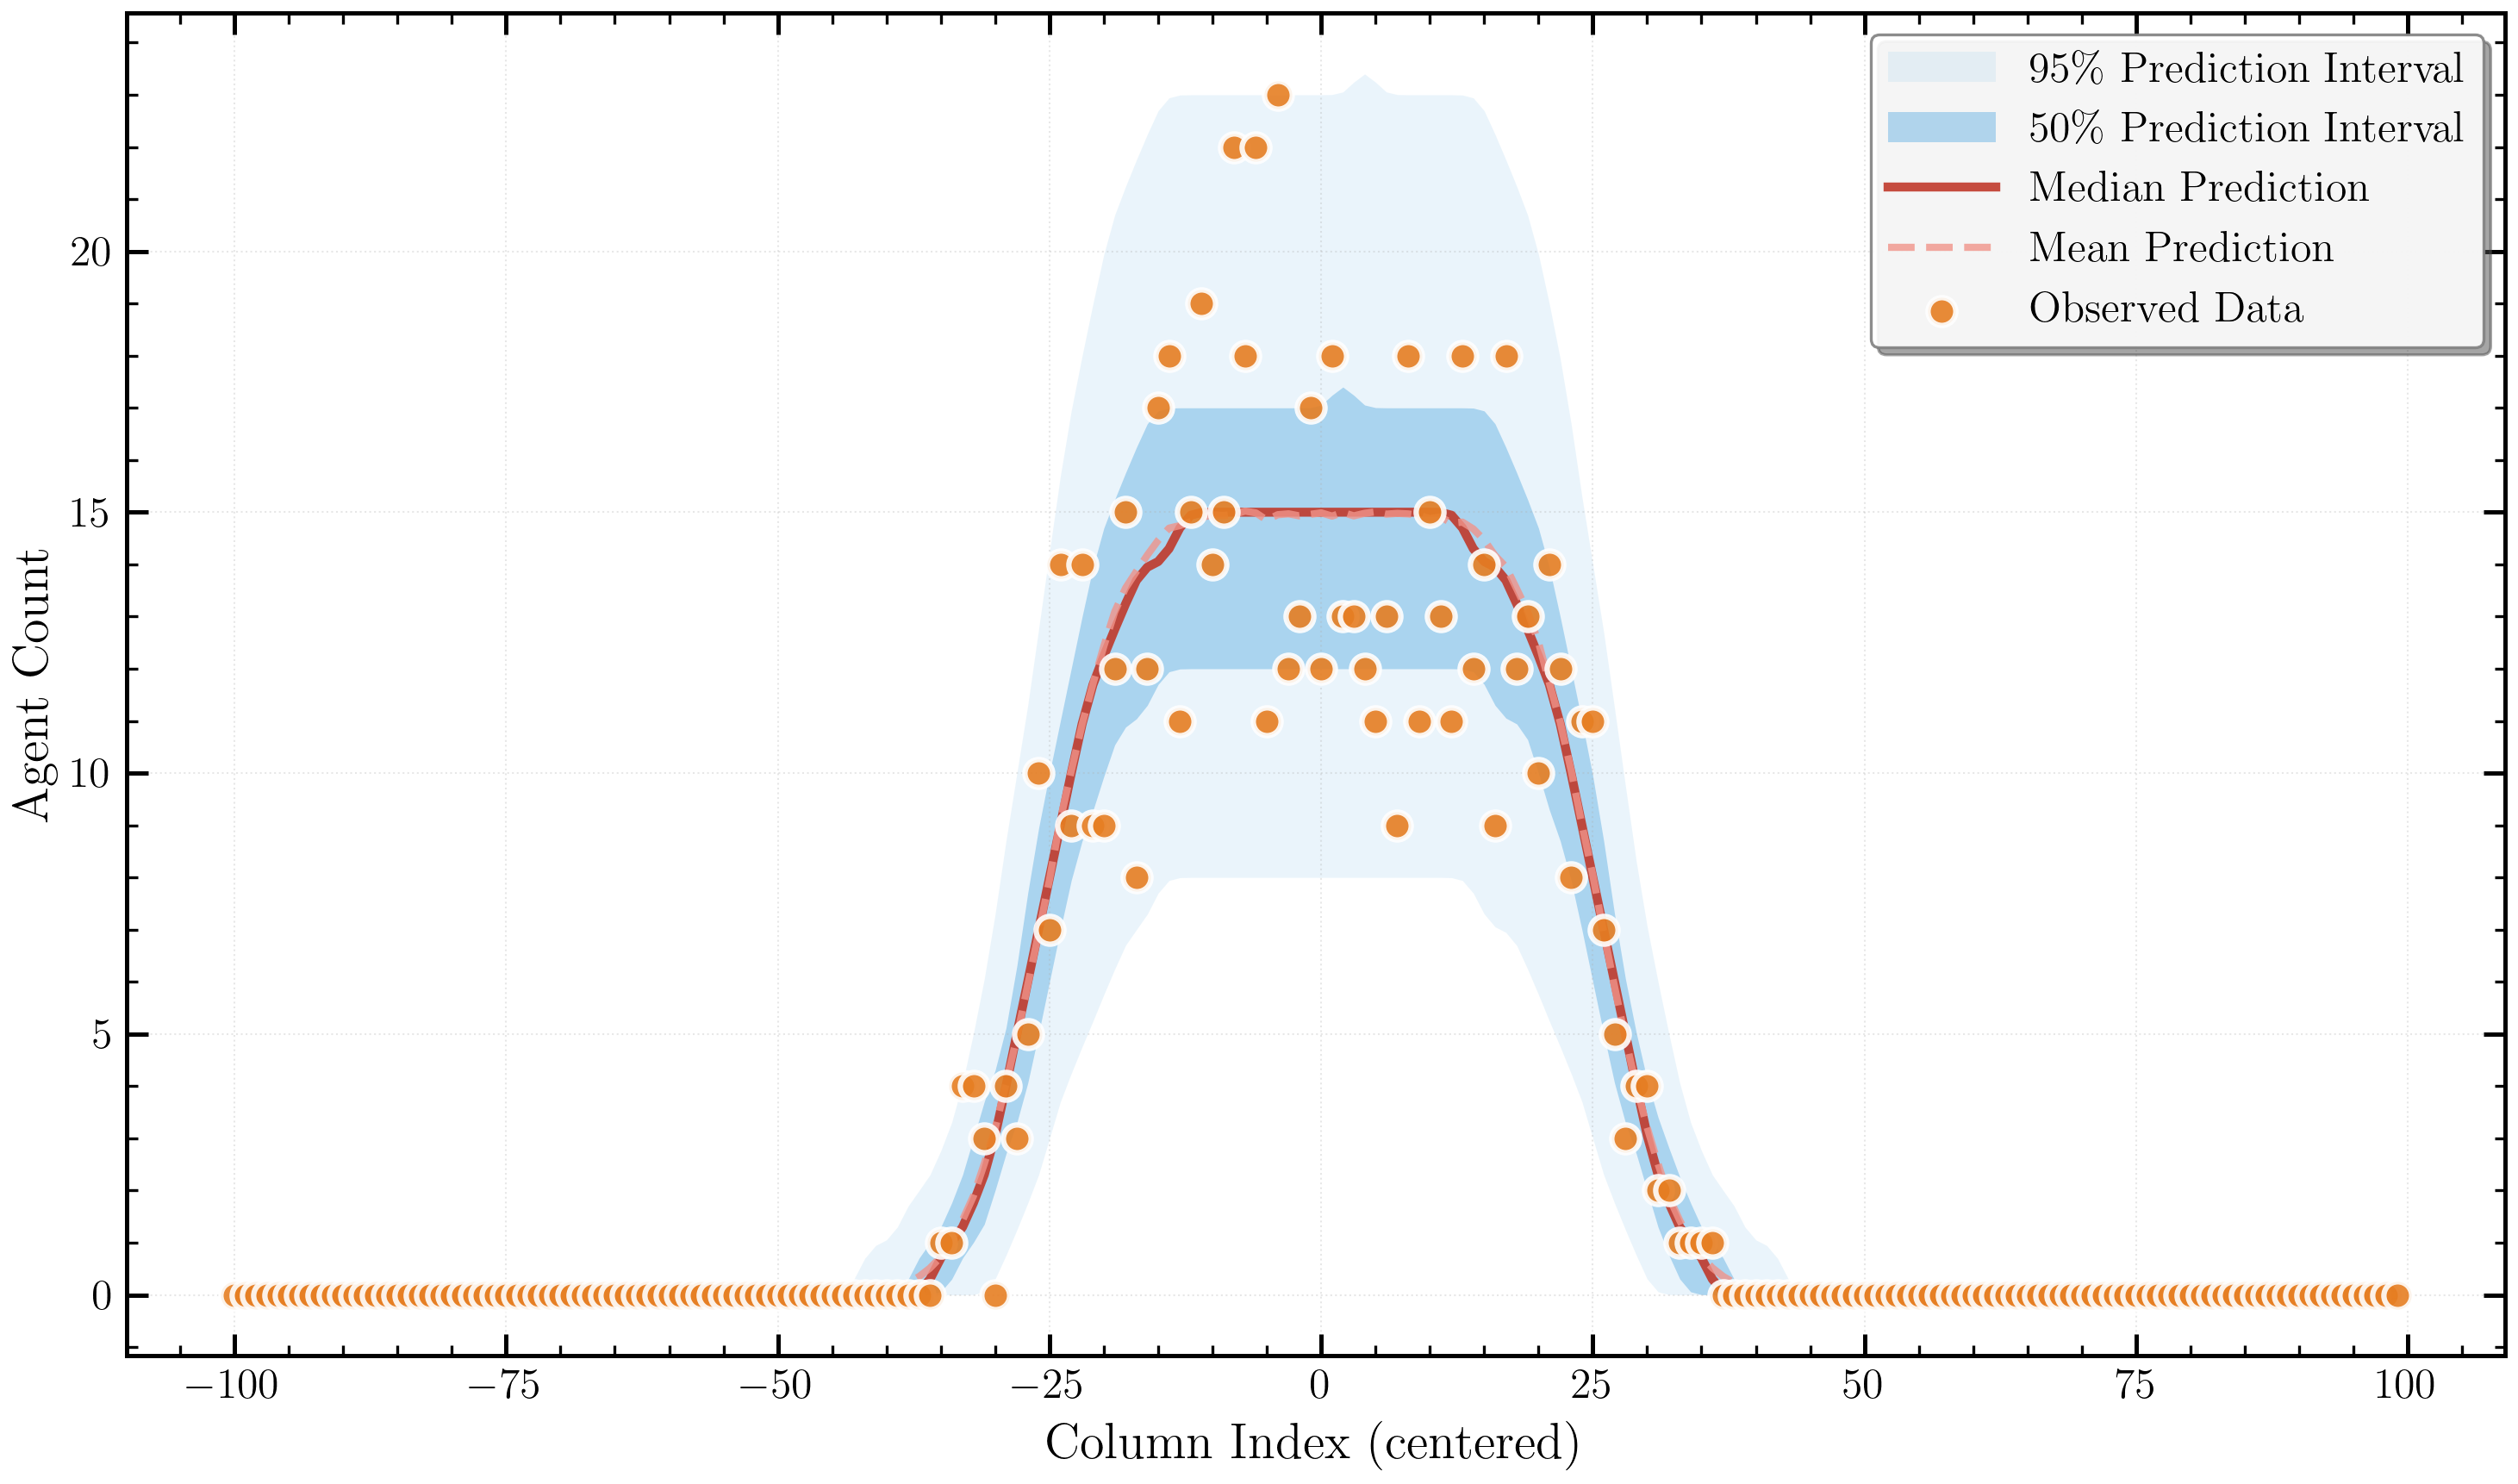
\includegraphics[width=0.8\textwidth]{images/example_predictive_plot_for_paper_1D}
	\caption{Posterior predictive checks from NPE using 1D column count data. The observed data (orange circles) is overlaid on predictions generated by simulating the model with parameters drawn from the inferred posterior distribution. The median (solid red line) and mean (dashed red line) of the predictions are shown, along with the 50\% (dark blue) and 95\% (light blue) prediction intervals. For visualization purposes, a Gaussian kernel has been applied to smooth the predictive distributions. The observed data points lie well within the 95\% prediction interval, indicating that the calibrated model is consistent with the data}
	\label{fig:npe_1d_predictive}
\end{figure}



\section{Learning from Raw Spatial Data}\label{sec:results_2d}

\subsection{Motivation for Full Spatial Data}

While column counts provide a natural summary of the spreading process, they necessarily discard information about the vertical distribution of agents. In principle, the spatial correlation structure within the 2D configuration contains additional information about the underlying parameters. For instance, clustering patterns, local density fluctuations, and spatial correlations may help distinguish between different combinations of $P$ and $U$ that produce similar column counts, cf. parameter identifiability, see Appendix \ref{ap:identifiability} \footnote{Although parameter identifiability is not a significant concern for the simple model we consider, additional spatial features are of interest for disentangling parameters in more complex models that incorporate processes like cell-cell adhesion or proliferation.}. Traditional inference methods require hand-crafted summary statistics, making it challenging to leverage such high-dimensional spatial information. NPE, however, can learn directly from raw data through automatic feature extraction. While the simple random walk models considered here are likely well-captured by 1D summary statistics, this approach demonstrates the broader potential of NPE for more complex biological systems where spatial structure is critical. For example, models incorporating agent-agent interactions, complex boundary conditions, spatially heterogeneous environments, or multi-species dynamics would generate spatial patterns that cannot be adequately summarized by simple column counts. In such cases, the ability to learn directly from full spatial data becomes essential for accurate parameter inference. Our framework provides a foundation that can be readily extended to these more sophisticated modeling scenarios without requiring manual specification of appropriate summary statistics.

\subsection{Architectural Adaptations for 2D Data}



Processing raw 2D spatial data requires a different architecture than the one used for 1D summary statistics. We treat each lattice configuration from the simulator as a binary image, where pixel values indicate the presence or absence of an agent. To learn informative features directly from this high-dimensional input, we replace the simple feed-forward network with a Convolutional Neural Network (CNN) \citep{lecun1998,krizhevsky2012,goodfellow2016}. The CNN acts as a powerful, learnable feature extractor that is embedded within the NPE pipeline. It uses a series of convolutional and pooling layers to progressively downsample the spatial data into a low-dimensional embedding. This process is designed to capture salient spatial features, such as clustering patterns and local agent densities, while preserving translational invariance. The learned embedding is then passed to the remainder of the network to estimate the posterior distribution. This end-to-end training ensures that the features extracted by the CNN are maximally informative for the specific task of parameter inference. A detailed specification of the CNN architecture, training parameters, and implementation details used in this work can be found in Appendix \ref{ap:cnn}.





\subsection{Parameter Inference from Raw Spatial Data}

Having established a baseline with 1D summary statistics, we now apply our NPE pipeline with the embedded CNN to perform inference directly on the raw 2D spatial data. This approach leverages the full spatial configuration of agents, aiming to extract additional information that may be lost when compressing the data into column counts.

\subsubsection{Experimental Setup}
The experimental setup remains identical to the 1D case, using the same synthetic observation generated with true parameters $P = 0.7$ ($D=0.7/4$) and $U = 0.3$. However, instead of using the 201-dimensional vector of column counts as input, the network now receives the full $50 \times 200$ binary image representing the agent locations on the lattice. We use the same broad uniform priors for $P$ and $U$ as before. Training details and architectural specifications for the CNN are provided in Appendix \ref{ap:cnn}.

\subsubsection{Parameter Inference Results}
Figure \ref{fig:npe_2d_posterior} shows the joint posterior distribution inferred from the 2D spatial data, overlaid with the result from the 1D column count analysis for direct comparison. The CNN-based approach recovers a posterior with means $D = 0.169^{+0.026}_{-0.023}$
 and $U = 0.290^{+0.008}_{-0.09}$. As summarised in Table \ref{tab:data_comparison}, leveraging the full spatial data yields a posterior with a precision that is highly comparable to that obtained using curated 1D summary statistics, cf. Section \ref{sec:1d_results}.

This result demonstrates that the CNN can automatically learn features from the raw data that are as informative as the carefully chosen summary statistics. This highlights a critical trade-off: the increased computational cost of training the CNN (Table \ref{tab:data_comparison}) must be weighed against the major advantage of avoiding manual feature engineering. For more complex models where optimal summary statistics are unknown, this direct-from-pixels approach may be advantageous for accurate inference.

\subsubsection{Predictive Performance}
We assess the predictive performance of the 2D-trained model using the same posterior predictive checking procedure as in Section \ref{sec:posterior_checks}. As shown in Figure \ref{fig:npe_2d_predictive}, the model generates predictions that are highly consistent with the observed data. The calibrated model accurately captures the spatial characteristics of the agent-based simulation, producing prediction intervals that are well-calibrated and physically consistent with the discrete nature of the data. Similar to the 1D case, the framework successfully captures the heteroscedastic nature of the uncertainty, demonstrating its robustness when applied to high-dimensional spatial inputs.

% --- Figures and Tables for this section ---

\begin{figure}[h]
	\centering
	\includegraphics[width=0.8\textwidth]{images/NPE_corner_plot_2d_D_v2}
	\caption{As Figure \ref{fig:npe_1d_posterior}, for posteriors generated from the NPE with CNN embedding networks, using full 2D spatial data.}
	\label{fig:npe_2d_posterior}
\end{figure}

\begin{figure}[h]
	\centering
	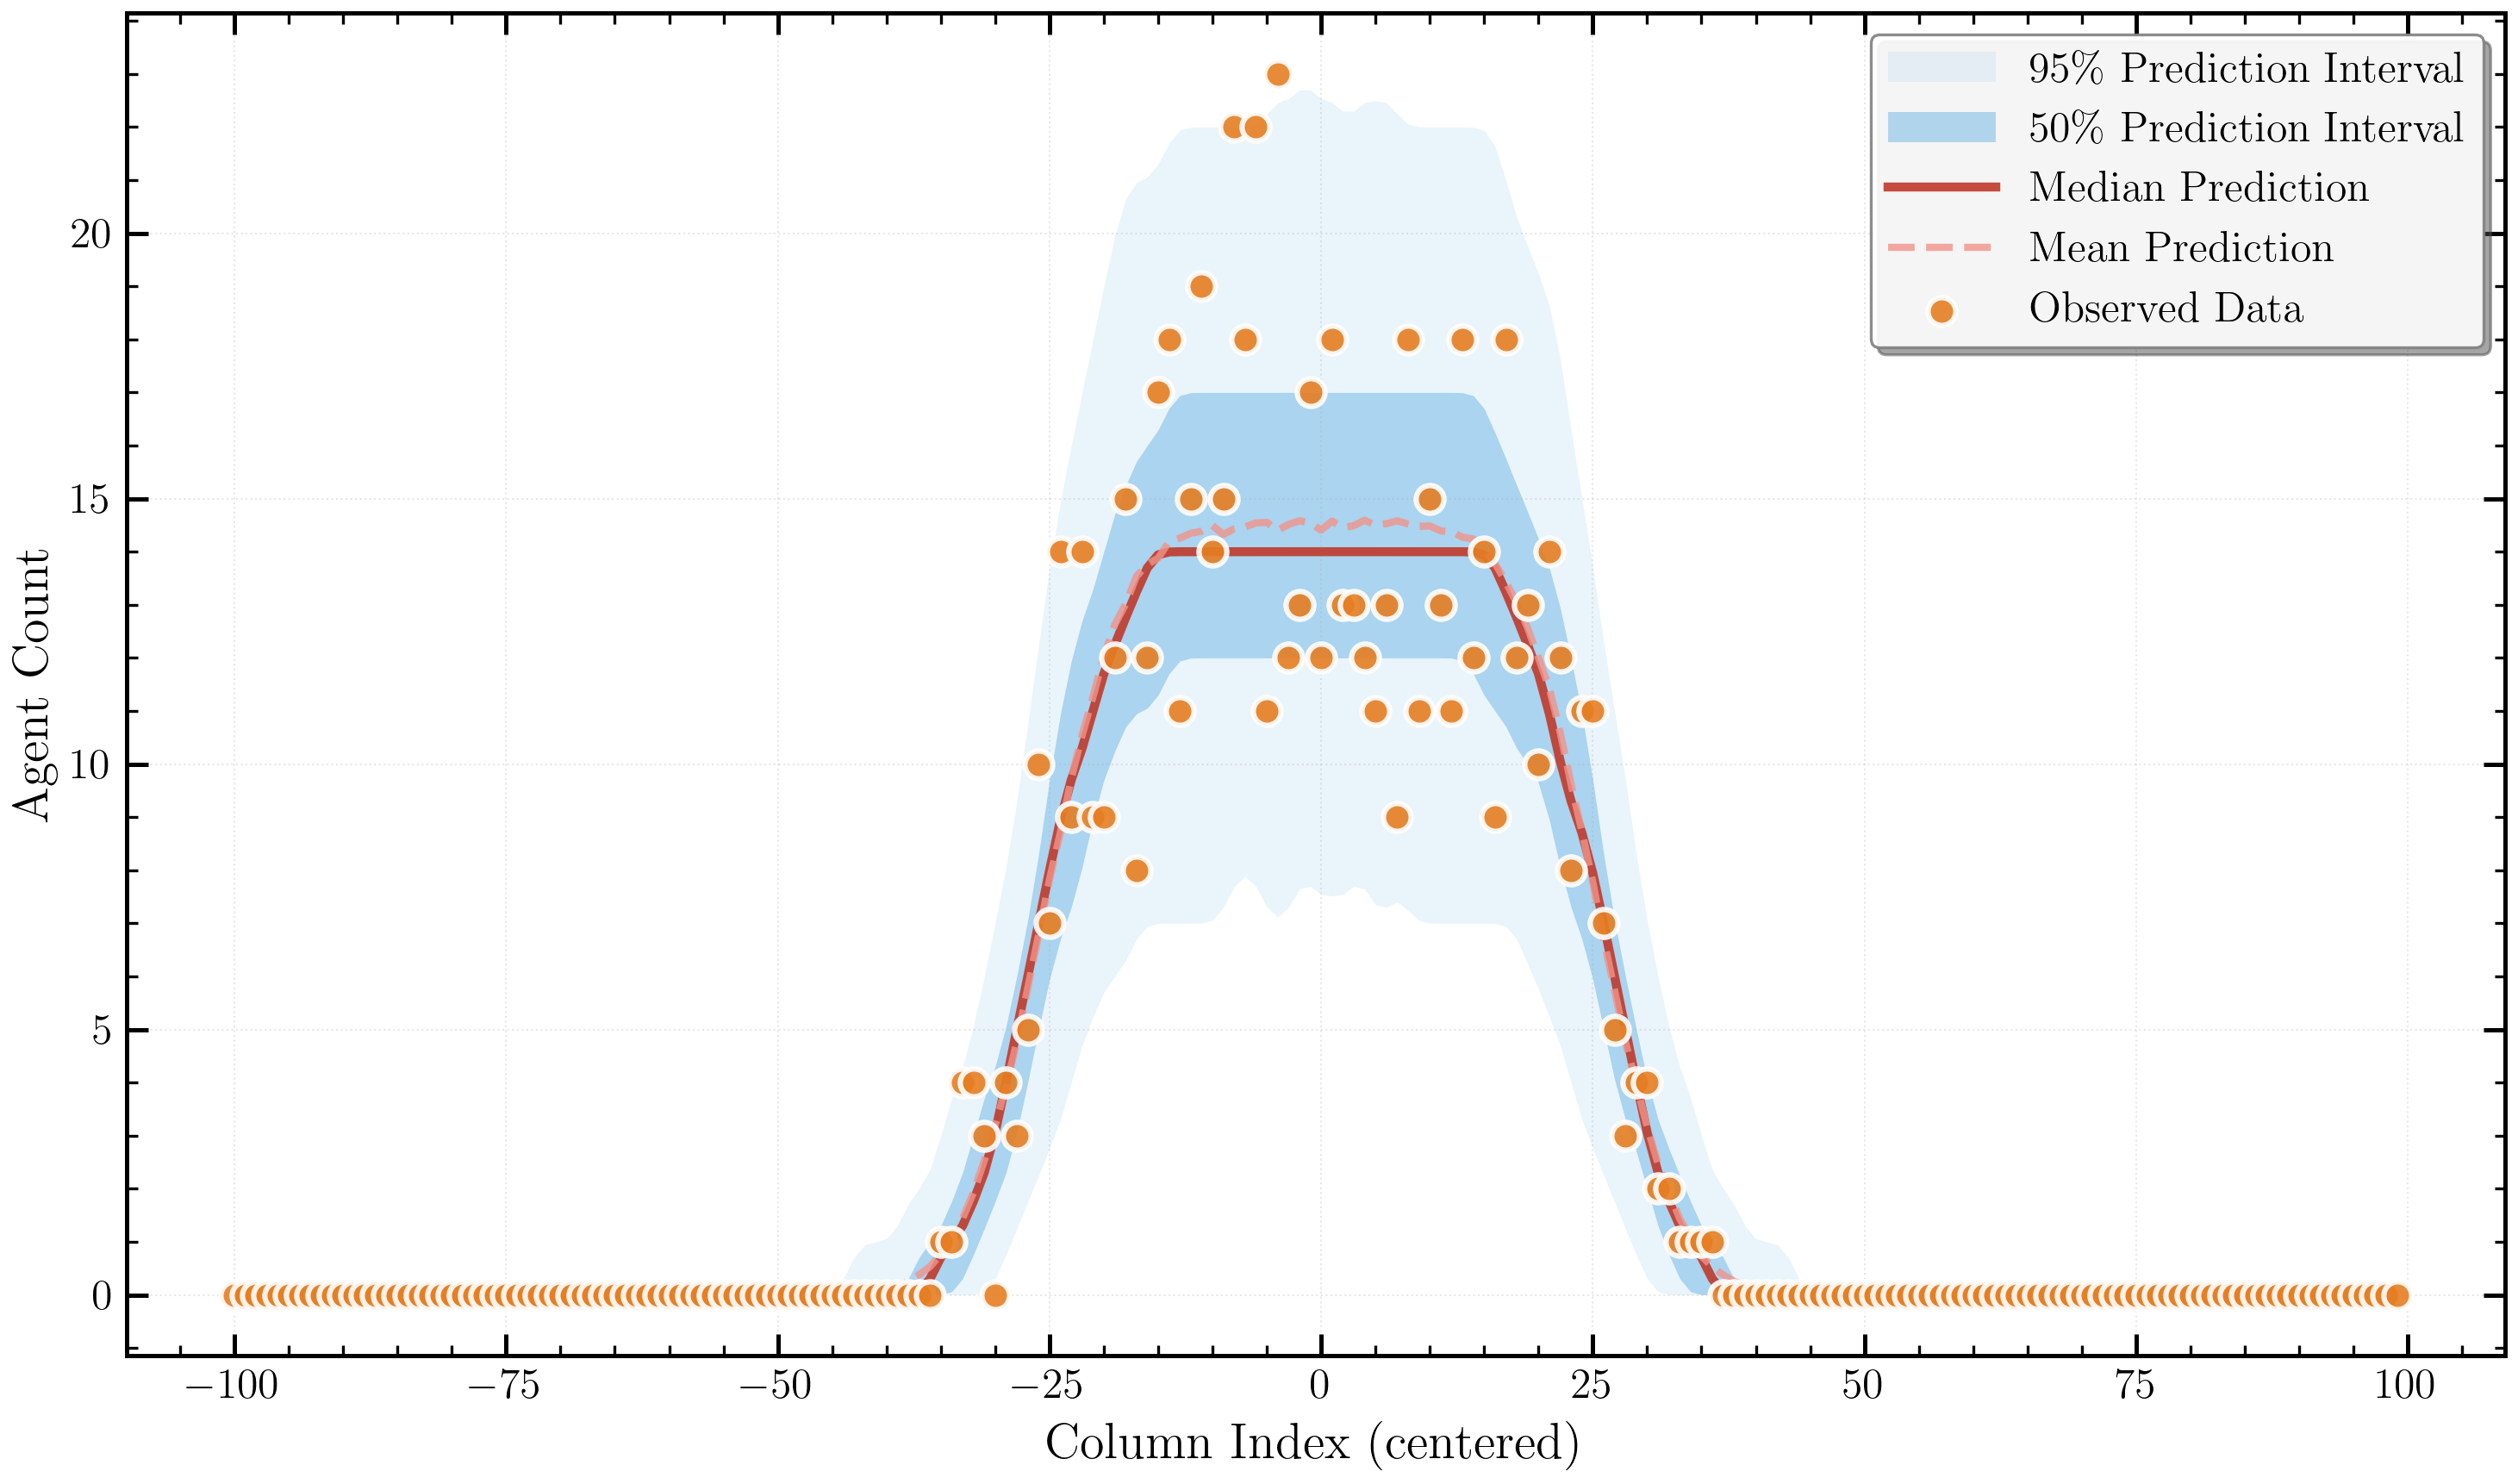
\includegraphics[width=0.8\textwidth]{images/example_predictive_plot_for_paper_2D}
	\caption{Posterior predictive check for the 2D spatial data model. The format is identical to Figure \ref{fig:npe_1d_predictive}. The predictions are well-calibrated and consistent with the observed data.}
	\label{fig:npe_2d_predictive}
\end{figure}


\begin{table}[h]
	\centering
	\begin{tabular}{lcc}
		\toprule
		\textbf{Data Type} & \textbf{Posterior for $D$} & \textbf{Posterior for $U$} \\
		\midrule
		1D Column counts & $0.164~[0.024, 0.024]$ & $0.298~[0.009, 0.008]$ \\
		2D Spatial data  & $0.169~[0.026, 0.023]$ & $0.290~[0.008, 0.009]$ \\
		\bottomrule
	\end{tabular}
	\caption{Comparison of NPE performance using different data representations. Posteriors are reported as the mean and the 95\% credible interval. Inference on the 2D spatial data provides comparable posterior precision to the 1D summary statistics.}
	\label{tab:data_comparison}
\end{table}







\section{Discussion}\label{sec:discussion}

\subsection{Advantages and Limitations of Neural Posterior Estimation}

NPE offers a robust and flexible framework for parameter inference, directly addressing several challenges that have limited the practical application of stochastic agent-based models. NPE eliminates the need for surrogate models by learning directly from the full stochastic simulator. This direct approach circumvents the systematic bias introduced by mean-field approximations and removes the challenging requirement of specifying explicit noise models that connect deterministic surrogates to stochastic observations. The method's ability to process raw high-dimensional data through automatic feature extraction represents another advantage, avoiding the information loss inherent in manually crafted summary statistics while enabling the analysis of complex spatial patterns that would be difficult to characterize a priori. The amortized nature of NPE provides substantial computational advantages once training is complete. After the initial investment in generating training data and optimizing the neural network, posterior inference for new observations requires only milliseconds of network evaluation rather than hours of simulation-based methods like ABC. This efficiency enables real-time analysis and interactive exploration of parameter space that would be prohibitive with classical approaches. Furthermore, normalizing flows can capture complex, multimodal posterior geometries that arise naturally from model non-identifiabilities without requiring restrictive parametric assumptions about posterior shape.

However, NPE also introduces new challenges and limitations that practitioners must carefully consider. The method's appetite for training data can be substantial, particularly for high-dimensional parameter spaces where the curse of dimensionality becomes prohibitive. Problems with more than 15-20 parameters may require simulation budgets that exceed practical computational limits. Additionally, NPE performance can degrade significantly when test observations fall outside the training distribution, making careful prior specification and robust training data generation critical for reliable inference.

The neural network architecture introduces another layer of complexity, as design choices regarding depth, width, and flow type can dramatically impact performance. Unlike classical methods with well-established theoretical foundations, NPE provides limited formal guarantees about convergence or approximation quality. This black-box nature can make diagnosis of poor performance challenging and requires practitioners to develop intuition about network behavior and training dynamics.




\subsection{Spatial information}

\textcolor{magenta}{TK: I think for these simple RW systems the CNN is probably overkill, but there are likely systems where spatial info becomes more useful. Need to query Jen/Mat for domain knowledge bio inputs here. The below bio examples are what I have been able to glean from scanning through papers, but maybe there are more appropriate examples. }


Our results highlight a critical trade-off between methodological complexity and computational cost. For the simple random walk model, well-chosen summary statistics provide comparable precision to the full spatial analysis at a fraction of the cost, making them a highly effective and efficient choice. However, this should not obscure the broader potential of spatial inference approaches; the cost-benefit calculation shifts decisively toward spatial approaches for more complex biological systems where crucial information is encoded in patterns that resist simple summarization, or where informative statistics are not known a priori.


In many realistic scenarios, crucial mechanistic information is encoded in intricate spatial patterns that are lost in simple one-dimensional projections. For example, models incorporating agent-agent interactions through exclusion effects, chemotaxis, or cell-cell adhesion generate complex formations that are lost when compressed into simple one-dimensional projections. Similarly, heterogeneous environments with spatially varying growth rates, physical barriers, or chemical gradients create complex spatial signatures that contain crucial parameter information. Multi-species dynamics involving competition, predation, or cooperation also produce emergent spatial organization that encodes information about underlying mechanisms. Collective behaviors such as swarming, flocking, or tissue morphogenesis involve coordinated movements that are fundamentally spatial phenomena requiring spatial analysis for proper characterization. In these more complex scenarios, CNN approaches would preserve information that would otherwise be discarded by traditional summary statistics. 



A critical aspect of applying deep learning models like CNNs in a scientific context is interpretability. While these networks are often treated as "black boxes", it is both possible and important to investigate the features they learn to solve a given inference problem. In principle, techniques such as activation mapping \cite{2023arXiv230914304M} or saliency maps \citep{2019arXiv191111293M} could be used to visualize the spatial features our CNN learns to associate with different parameter values.  One might expect the network to develop sensitivity to biologically relevant patterns like the sharpness of the spreading front, local cell density gradients, or the degree of cell clustering. By identifying these learned features, a researcher could validate that the network's reasoning aligns with established biological theory, or discover novel spatial statistics that are informative but not immediately obvious to a human observer. While a detailed feature analysis is beyond the scope of this work, we highlight its importance for future applications. The ability to not only perform inference but also to extract the learned representations that enable it is a key advantage of this approach. 

The ability to perform inference with stochastic models on spatiotemporal data has direct implications for experimental design. Traditional protocols often reduce rich data from sources like time-lapse microscopy to simplified measurements. This is a compromise driven by past computational limits, not biological necessity. Our framework removes this barrier, enabling direct analysis that preserves the full spatial information. This should encourage the strategic collection and retention of rich datasets, which is crucial for improving parameter identifiability in complex systems where spatial structure encodes mechanistic information. \textcolor{magenta}{TK: perhaps experimentalists already do this. Again, need domain knowledge.}




\subsection{Computational Scalability and Future Directions}
The NPE framework, particularly with the CNN-based spatial analysis, introduces several computational considerations that will influence its applicability to large-scale problems.

The primary cost for any NPE approach is the upfront simulation budget, which can become substantial for models with high-dimensional parameter spaces ($> 15-20$ parameters). On top of this, the CNN adds specific challenges; (i) memory requirements scale quadratically with spatial resolution, potentially limiting application to very high-resolution imaging data without careful optimization; (ii) architecture selection for CNN embedding networks requires problem-specific tuning of depth, width, and kernel sizes, adding complexity to the analysis pipeline; (iii) the combined optimization of feature extraction and density estimation can be more challenging than simpler approaches, requiring careful hyperparameter selection and potentially longer training times.

Despite these challenges, several technological trends suggest that spatial inference approaches will become increasingly practical. Advances in GPU computing and specialized hardware for neural network training continue to reduce computational barriers. Improved network architectures and training algorithms may reduce the simulation budgets required for reliable inference. Transfer learning approaches could enable pre-trained spatial feature extractors to be adapted to new biological problems with reduced computational cost.

The framework developed here provides a foundation that can evolve with these technological advances while addressing increasingly complex biological questions. Future extensions might incorporate three-dimensional spatial data, temporal dynamics, or multi-modal observations combining spatial patterns with biochemical measurements. As biological modeling advances toward more realistic representations of complex systems, the ability to learn directly from high-dimensional, spatially structured data will become essential for extracting quantitative insights from biological observations.


\section{Conclusion}

\textcolor{magenta}{TK: TBD}

\appendix






\newpage
\section{Synthetic data generation}\label{sec: synthetic_data_generation}

\textcolor{magenta}{TK: TBD}

The experimental configuration consists of a two-dimensional lattice with dimensions $H = 50$ and $W = 200$, where agents are initially placed within the region $|x| \leq 25$ with probability $U = 0.5$. The system evolves for 100 time steps with movement probability $P$ and proliferation probability $R$, corresponding to macroscopic diffusivity $D = P\Delta^2/(4\tau)$ and growth rate $r = R/\tau$ in the continuum limit.



\section{Identifiability}\label{ap:identifiability}

\textcolor{magenta}{TK: TBD. Perhaps a short discussion on identifiability either here or in main text body. Might be out of scope.}

\section{NPE Implementation}\label{ap:npe_implementaion}

\textcolor{magenta}{TK: TBD. Could also point to config files in repo for reproducibility}

Our specific implementation choices include:
\begin{itemize}
	\item \textbf{Flow architecture:} Neural spline flows with 5 coupling layers, 10 bins per spline, and embedding networks of 2 hidden layers with 50 units each.
	\item \textbf{Training:} Adam optimizer with learning rate $10^{-4}$, batch size 512, and early stopping based on validation loss.
	\item \textbf{Validation:} 20\% of simulations reserved for validation, with training stopped when validation loss increases for 10 consecutive epochs.
\end{itemize}



\section{CNN implementation} \label{ap:cnn}

\textcolor{magenta}{TK: TBD.}



Our CNN architecture consists of:

\begin{itemize}
	\item \textbf{Convolutional layers:} Three convolutional layers with 32, 64, and 128 filters respectively, each with $3 \times 3$ kernels, followed by ReLU activations and $2 \times 2$ max pooling operations.
	
	\item \textbf{Dimensionality reduction:} The CNN compresses the $H \times W = 10,000$ dimensional input to a 256-dimensional embedding that captures relevant spatial features while remaining computationally tractable.
	
	\item \textbf{Fully connected layers:} The flattened convolutional features are passed through two fully connected layers (512 and 256 units) with ReLU activations and dropout (rate = 0.3) for regularization.
	
	\item \textbf{Translation invariance:} The convolutional architecture naturally handles the translation-invariant nature of the spreading process, learning features that are consistent across spatial locations.
\end{itemize}


Training NPE with 2D data requires several adjustments compared to the 1D case:

\begin{itemize}
	\item \textbf{Increased simulation budget:} Due to the higher-dimensional input space, we use 15,000 simulations per SNPE round (compared to 10,000 for 1D) to ensure adequate coverage of the joint parameter-data space.
	
	\item \textbf{Extended training time:} The CNN embedding network requires additional optimization iterations. We use a learning rate of $5 \times 10^{-5}$ with batch size 256, training for up to 500 epochs with early stopping.
	
	\item \textbf{Memory considerations:} Each 2D observation requires significantly more memory ($50 \times 200 = 10,000$ values vs. 201 for column counts), necessitating careful batch size selection and data loading strategies.
\end{itemize}




\bibliographystyle{plain}
\bibliography{references}  

\end{document}
